\section{测试结果}

\subsection{单元测试}

\paragraph{数据预处理与语义分割模块}
\par 该模块的测试方法及测试结果见表\ref{unit_test_result1}。
\begin{table}[H]
	\centering
	\caption{数据预处理与语义分割模块测试用例表}
	\label{unit_test_result1}
	\begin{tabular}{p{0.5cm}p{3.1cm}p{5.2cm}p{1.8cm}p{1.9cm}}
		\toprule
		\multicolumn{1}{c}{编号}      & \multicolumn{1}{c}{前置条件} & \multicolumn{1}{c}{测试步骤} & \multicolumn{1}{c}{预期结果} & \multicolumn{1}{c}{实际结果} \\
		\midrule
		\centering\arraybackslash 1 & 图像帧数据可用                  & 从指定源读取图像帧数据并计时           & > 30 帧/秒                 & 166.7 帧/秒                \\
		\centering\arraybackslash 2 & 获得原始图像数据                 & 验证输出图像是否具有正确的格式和归一化数值    & 格式及数值正确                  & 格式及数值正确                  \\
		\centering\arraybackslash 3 & 获得原始图像数据                 & 验证输出图像的尺寸和内容是否符合要求       & 尺寸及内容正确                  & 部分尺寸及内容正确                \\
		\centering\arraybackslash 4 & 获得预测结果和真实结果              & 计算语义分割的 mIoU 值             & > 60\%                   & 82.1\%                  \\
		\bottomrule
	\end{tabular}
\end{table}

\par 图像帧读取速度为166.7帧/秒,超过RGB-D相机帧速率(约 30 帧/秒)。
所有图像成功转换至目标格式,像素数据成功归一化至目标范围。
图像裁剪与缩放的成功率为97.4\%,scene0088\_03, scene0144\_00, scene0144\_01, scene0354\_00, scene0474\_03, scene0689\_00, scene0704\_00和scene0704\_01 场景输出图像的尺寸不符合要求,
其他场景的RGB图像和语义分割图像均缩放至$1296 \times 968$,深度图像均缩放至$640 \times 480$,图像预处理效果满意。
\par 使用DeepLab2官方提供的kMaX-DeepLab模型以Axial-ResNet-50(MaX-S w/ GeLU)作为骨干网络,在Cityscapes train-fine数据集进行150000 Epochs的训练后,语义分割的mIoU结果能够达到82.1\%\cite{kmax_deeplab_result},足够应对大多数场景的语义理解需求。

\paragraph{位姿估计与场景管理模块}
\par 该模块的测试方法及测试结果见表\ref{unit_test_result2}。
\begin{table}[H]
	\centering
	\caption{位姿估计与场景管理模块用例表}
	\label{unit_test_result2}
	\begin{tabular}{p{0.5cm}p{4.1cm}p{3.8cm}p{1.6cm}p{2.5cm}}
		\toprule
		\multicolumn{1}{c}{编号}      & \multicolumn{1}{c}{前置条件} & \multicolumn{1}{c}{测试步骤} & \multicolumn{1}{c}{预期结果}            & \multicolumn{1}{c}{实际结果}        \\
		\midrule
		\centering\arraybackslash 5 & 获得估计结果和真实结果              & 计算位姿矩阵综合误差               & \centering\arraybackslash < 5\%     & \centering\arraybackslash 3\%   \\
		\centering\arraybackslash 6 & 空间划分方法已定义                & 检查网格序号计算结果               & \centering\arraybackslash 100\%     & \centering\arraybackslash 100\% \\
		\centering\arraybackslash 7 & 点云参数已设置                  & 计算InitData执行时间           & \centering\arraybackslash < 5000 ms & 1752 ms / 113 ms                \\
		\bottomrule
	\end{tabular}
\end{table}
\par 位姿估计的精度在所有测试场景中均可以达到 3\% 的误差范围内,场景空间的划分和更新成功率为100\%,点云对象初始化速度为1752 ms / 113 ms。
使用PCI Express(PCIe)在CPU-GPU间数据传输速率达到 8 GT/s,如图\ref{fig:cpugpu}所示,满足实时性要求。

\begin{figure}[htbp]
	\centering
	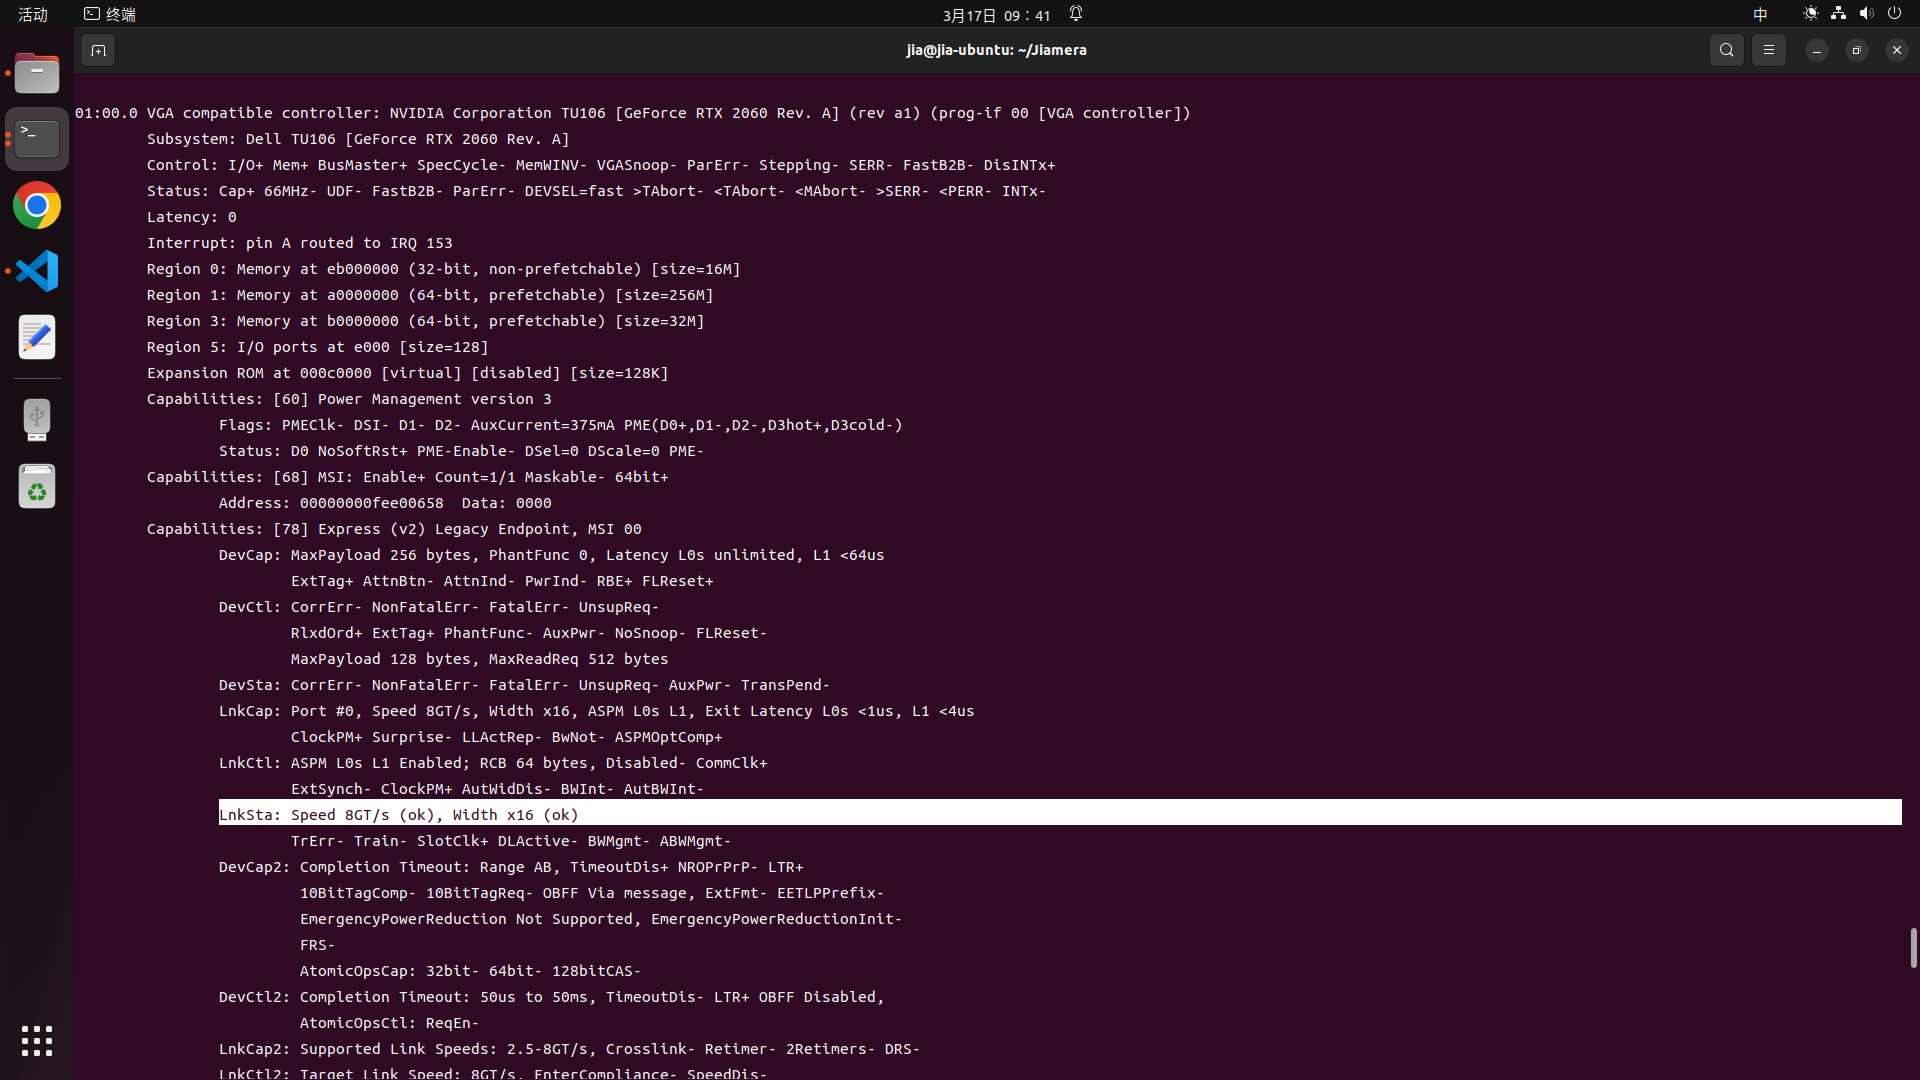
\includegraphics[width=1\textwidth]{figures/test_para/pcie_5cm.png}
	\caption{CPU-GPU数据传输速率}
	\label{fig:cpugpu}
	\note{注:LnkSta是Link Status的缩写,表示连接的状态。Speed 8GT/s (ok)表示当前连接的速度是8千兆/秒。Width x16 (ok)表示当前连接的宽度是16个数据通道。16条并行数据传输是PCI Express架构的最大配置。}
\end{figure}

\paragraph{点云生成与语义融合模块}
\par 该模块的测试方法及测试结果见表\ref{unit_test_result3}。
\begin{table}[h]
	\centering
	\caption{点云生成与语义融合模块用例表}
	\label{unit_test_result3}
	\begin{tabular}{p{0.5cm}p{3.5cm}p{5.1cm}p{1.2cm}p{2.2cm}}
		\toprule
		\multicolumn{1}{c}{编号}       & \multicolumn{1}{c}{前置条件}            & \multicolumn{1}{c}{测试步骤} & \multicolumn{1}{c}{预期结果}          & \multicolumn{1}{c}{实际结果}                  \\
		\midrule
		\centering\arraybackslash 8  & 获得输入图像数据                            & 记录每帧处理所需时间               & \centering\arraybackslash < 33 ms  & \centering\arraybackslash 13 ms / 1 ms    \\
		\midrule
		\centering\arraybackslash 9  & \multirow{3}{3.5cm}{三维重建及语义融合完成}    & 计算语义分割的 mIoU 正确率         & \centering\arraybackslash > 50\%  & \centering\arraybackslash 51\% / 42\%     \\
		\centering\arraybackslash 10 &                                     & 计算平均每帧的像素使用率             & \centering\arraybackslash > 30\%  & \centering\arraybackslash 82.4\% / 5.3\%  \\
		\centering\arraybackslash 11 &                                     & 计算点云模型的点云使用率             & \centering\arraybackslash > 0.5\% & \centering\arraybackslash 0.11\% / 0.24\% \\
		\midrule
		\centering\arraybackslash 12 & \multirow{2}{3.5cm}{ 使用点云多采样进行语义融合} & 计算语义分割的 mIoU 正确率         & \centering\arraybackslash > 5\%   & \centering\arraybackslash 8.2\% / 5.4\%   \\
		\centering\arraybackslash 13 &                                     & 记录每帧处理所需时间               & \centering\arraybackslash < 200\% & \centering\arraybackslash 540\% / 680\%   \\
		\midrule
		\centering\arraybackslash 14 & 对输出模型滤波降噪                           & 计算语义分割的 mIoU 正确率         & \centering\arraybackslash > 10\%  & \centering\arraybackslash 5.5\% / 7.2\%   \\
		\bottomrule
	\end{tabular}
\end{table}

\par 每帧处理速度为13 ms / 1 ms,完全符合室内场景重建的要求,但是由于TSDF算法固有特性,对于表面细节的表达能力有限,且产生较严重的拖尾现象。
\par 使用自行编写的 EvaluateSegmentation 脚本评估语义分割的正确率,它计算了每个场景的预测模型与Ground Truth模型的IoU值,以及所有场景的mIoU值,伪代码如算法\ref{algo:EvaluateSemanticSegmentation}所示。
表\ref{miou_2cm}记录了不同标签在所有测试场景中的IoU值。结果显示,所有标签在所有场景下的mIoU值达到51\% / 42\%,与 PanopticFusion、Online SegFusion 等算法基本持平。

\begin{table}[htbp]
	\centering
	\caption{语义分割IoU结果}
	\label{miou_2cm}
	\begin{tabular}{cccccccc}
		\toprule
		方法               & average       & wall          & floor         & cabinet       & bed           & chair         & sofa          \\
		\midrule
		ours(2cm)        & 0.51          & 0.48          & 0.67          & \textbf{0.47} & 0.48          & 0.55          & 0.56          \\
		ours(5cm)        & 0.42          & 0.42          & 0.67          & 0.44          & 0.50          & 0.52          & 0.40          \\
		PointNet++       & 0.34          & 0.52          & 0.67          & 0.26          & 0.48          & 0.36          & 0.37          \\
		PointCNN         & 0.46          & \textbf{0.71} & \textbf{0.95} & 0.32          & 0.61          & 0.71          & 0.55          \\
		PanopticFusion   & 0.53          & 0.60          & 0.82          & 0.39          & \textbf{0.69} & \textbf{0.63} & \textbf{0.65} \\
		Online SegFusion & 0.52          & 0.70          & 0.76          & 0.43          & 0.64          & \textbf{0.63} & 0.56          \\
		\toprule
		方法               & table         & door          & window        & bookshelf     & picture       & counter       &               \\
		\midrule
		ours(2cm)        & 0.44          & \textbf{0.53} & 0.52          & 0.49          & 0.47          & \textbf{0.38} &               \\
		ours(5cm)        & \textbf{0.51} & 0.51          & 0.51          & 0.49          & \textbf{0.48} & 0.35          &               \\
		PointNet++       & 0.23          & 0.26          & 0.25          & 0.46          & 0.12          & 0.25          &               \\
		PointCNN         & 0.46          & 0.32          & 0.48          & 0.36          & 0.17          & 0.30          &               \\
		PanopticFusion   & 0.44          & 0.29          & \textbf{0.56} & 0.60          & 0.24          & 0.23          &               \\
		Online SegFusion & 0.45          & 0.41          & 0.51          & \textbf{0.58} & 0.17          & 0.35          &               \\
		\bottomrule
	\end{tabular}
	\note{注:数据来自https://kaldir.vc.in.tum.de/scannet\_benchmark/}

\end{table}

\par 像素使用率分别为82.4\% / 5.3\%,点云使用率分别为0.11\% / 0.24\%,这表明系统在创建和使用点云对象、图像帧方面的效率有待提高。
\par 多采样反走样操作在更高分辨率下对语义分割有更大的提升,但是会显著降低系统运行速度;而滤波降噪对语义分割正确率有一定提升,且影响相对较小。

\paragraph{可视化模块} \label{vis_test}
\par 该模块的测试方法及测试结果见表\ref{unit_test_result4}。
\begin{table}[H]
	\centering
	\caption{可视化模块用例表}
	\label{unit_test_result4}
	\begin{tabular}{p{0.5cm}p{3.5cm}p{4.1cm}p{2.2cm}p{2.2cm}}
		\toprule
		\multicolumn{1}{c}{编号}       & \multicolumn{1}{c}{前置条件} & \multicolumn{1}{c}{测试步骤} & \multicolumn{1}{c}{预期结果}          & \multicolumn{1}{c}{实际结果}        \\
		\midrule
		\centering\arraybackslash 15 & GLFW 库已安装                & 检查是否弹出动画窗口               & \centering\arraybackslash 成功初始化   & \centering\arraybackslash 部分初始化 \\
		\centering\arraybackslash 16 & OpenGL正常工作               & 查看性能检测工具                 & \centering\arraybackslash 利用率合理   & \centering\arraybackslash 利用率合理 \\
		\centering\arraybackslash 17 & 用户输入指令                   & 测量响应时间                   & \centering\arraybackslash < 5 ms  & \centering\arraybackslash < 1 ms \\
		\centering\arraybackslash 18 & 动画正常播放                   & 计算每帧耗时                   & \centering\arraybackslash < 50 ms & \centering\arraybackslash 16 ms \\
		\bottomrule
	\end{tabular}
\end{table}

\par GLFW窗口初始化成功率为66\%,这是由于Linux系统中OpenGL的单线程渲染限制和状态机设计在多线程环境中产生的竞争问题\cite{linux_kernel,MultiThreadingVulkan}。GPU显存利用率分别为92.7\% / 10.3\%,帧缓冲区大小分别为5.4GB /
691.2MB,同时使用\texttt{glfwWindowHint(GLFW\_DOUBLEBUFFER, GLFW\_TRUE)}设置双缓冲,确保了动画的流畅度。 用户输入响应延迟小于1 ms,动画同步延迟 < 1 ms,帧率为16 ms/帧,满足实时交互的要求。

\paragraph{模型导入导出模块}
\par 该模块的测试方法及测试结果见表\ref{unit_test_result5}。
\begin{table}[htbp]
	\centering
	\caption{模型导入导出模块用例表}
	\label{unit_test_result5}
	\begin{tabular}{p{0.5cm}p{4.1cm}p{3.4cm}p{2cm}p{2.5cm}}
		\toprule
		\multicolumn{1}{c}{编号}       & \multicolumn{1}{c}{前置条件}               & \multicolumn{1}{c}{测试步骤} & \multicolumn{1}{c}{预期结果}          & \multicolumn{1}{c}{实际结果}                \\
		\midrule
		\centering\arraybackslash 19 & \multirow{2}{4.1cm}{已生成 PLY 格式的点云数据文件} & 查看数据文件大小                 & \centering\arraybackslash < 5MB   & \centering\arraybackslash 3.5MB / 601KB \\
		\centering\arraybackslash 20 &                                        & 记录读取和导出时间                & \centering\arraybackslash < 5秒/MB & \centering\arraybackslash < 2秒/MB       \\
		\bottomrule
	\end{tabular}
\end{table}
\par PLY点云数据文件平均大小为 3.5 MB / 601 KB,平均读取速度为 1 秒/MB,导出速度为 2 秒/MB。RGB信息和语义信息均成功导出,导出模型的位姿与Ground Truth模型完全重叠。
更多导出效果如附录中图\ref{fig:scene0011_00_result}、图\ref{fig:scene0030_00_result}、图\ref{fig:scene0500_00_result}和图\ref{fig:scene0518_00_result}所示。

\subsection{集成测试}
测试方法及测试结果见表\ref{unit_test_result}。
\begin{table}[H]
	\centering
	\caption{集成测试用例表}
	\label{unit_test_result}
	\begin{tabular}{p{0.5cm}p{3.2cm}p{5cm}p{1.5cm}p{2.3cm}}
		\toprule
		\multicolumn{1}{c}{编号}      & \multicolumn{1}{c}{前置条件}                 & \multicolumn{1}{c}{测试步骤}                    & \multicolumn{1}{c}{预期结果}         & \multicolumn{1}{c}{实际结果}                  \\
		\midrule
		\centering\arraybackslash 21 & \multirow{3}{3.2cm}{系统已成功安装,并设置正确的点云分辨率} & \multirow{3}{5cm}{启动系统,观测性能监视器}             & \centering\arraybackslash < 80\% & \centering\arraybackslash 33.7\% / 61.5\% \\
		\centering\arraybackslash 22 &                                          &                                             & \centering\arraybackslash > 50\% & \centering\arraybackslash 26\% / 55\%     \\
		\centering\arraybackslash 23 &                                          &                                             & \centering\arraybackslash < 50\% & \centering\arraybackslash 34.4\% / 4.6\%  \\
		\midrule
		\centering\arraybackslash 24 & \multirow{2}{3.2cm}{系统已安装在相应的操作系统平台上}    & \multirow{2}{5cm}{启动系统,检查是否存在依赖项缺失、界面显示等问题} & \centering\arraybackslash 无异常    & \centering\arraybackslash 无异常             \\
		\centering\arraybackslash 25 &                                          &                                             & \centering\arraybackslash 无异常    & \centering\arraybackslash 部分异常            \\
		\midrule
		\centering\arraybackslash 26 & 系统已成功安装                                  & 选择不同规模的场景,启动系统,检查系统是否正常运行                   & \centering\arraybackslash 正常运行   & \centering\arraybackslash 正常运行            \\
		\centering\arraybackslash 27 & 系统已成功安装                                  & 启动系统并长时间运行,检查内存是否稳定                         & \centering\arraybackslash 内存稳定   & \centering\arraybackslash 内存稳定            \\
		\centering\arraybackslash 28 & 系统已成功安装                                  & 设置不同的点云分辨率,启动系统,检查系统是否正常运行                  & \centering\arraybackslash 正常运行   & \centering\arraybackslash 部分正常运行          \\
		\bottomrule
	\end{tabular}
\end{table}

\paragraph{性能占用}

\par 图\ref{fig:2cm_result}和图\ref{fig:5cm_result}所示,在2cm / 5cm分辨率的重建过程中,系统的CPU(8核)占用率为270\% / 492\%。GPU占用率为26\% / 55\%,内存占用率为34.4\% / 4.6\%,没有对系统造成过重负荷。
需要注意的是,较低的点云分辨率意味着 GPU 计算量更低,每帧重建速度更快,导致 CPU 和 GPU 以更高的占用率运行。

\begin{figure}[htbp]
	\centering
	\subfigure[CPU]{
		\begin{minipage}[t]{0.48\linewidth}
			\centering
			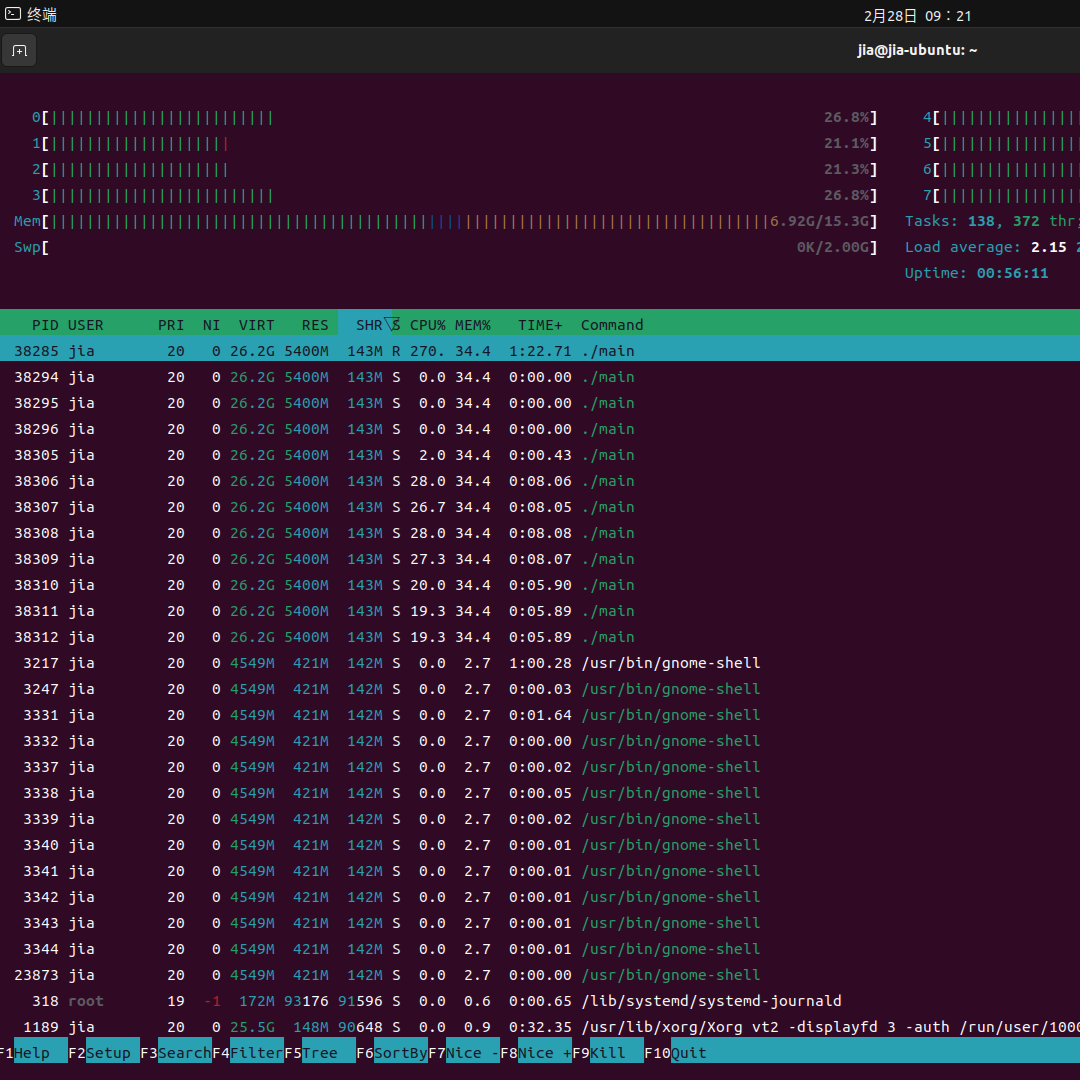
\includegraphics[width=1\textwidth]{figures/test_para/2cm_cpu.png}
		\end{minipage}
	}
	\subfigure[GPU]{
		\begin{minipage}[t]{0.48\linewidth}
			\centering
			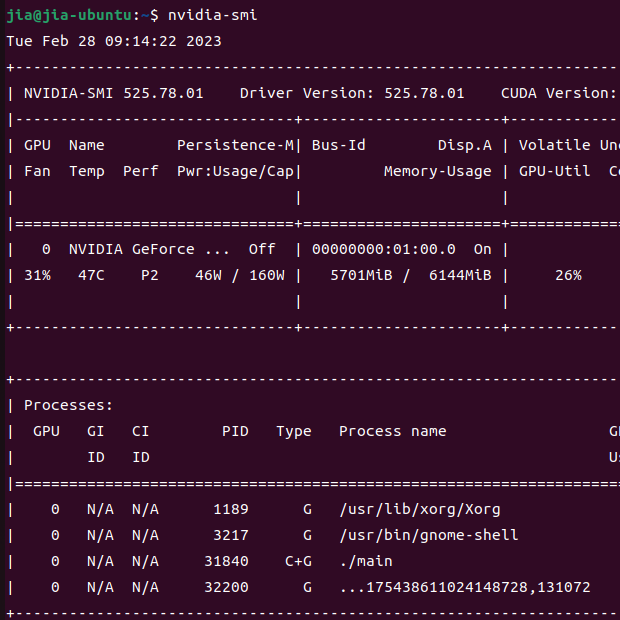
\includegraphics[width=1\textwidth]{figures/test_para/2cm_gpu.png}
		\end{minipage}
	}
	\caption{2cm点云分辨率性能占用}
	\label{fig:2cm_result}
	\note{注:CPU性能测试使用Linux的htop命令,它提供了系统的实时视图,包括正在运行的进程以及对系统资源的使用情况。其中,PRI是进程的优先级,数字越低,优先级越高。NI是nice值,用来影响进程的调度优先级。VIRT是进程的虚拟内存总量。RES是进程正在使用的物理内存量。SHR是共享内存大小,这部分内存可以被其他进程共享使用。S代表进程的状态,R表示正在运行或者在运行队列中等待。TIME+是进程消耗的CPU时间总和,格式为min:sec。GPU性能测试使用NVIDIA System Management Interface工具,使用方法参考\href{https://developer.nvidia.com/nvidia-system-management-interface}{官方文档:developer.nvidia.com/nvidia-system-management-interface}。}
\end{figure}

\begin{figure}[htbp]
	\centering
	\subfigure[CPU]{
		\begin{minipage}[t]{0.48\linewidth}
			\centering
			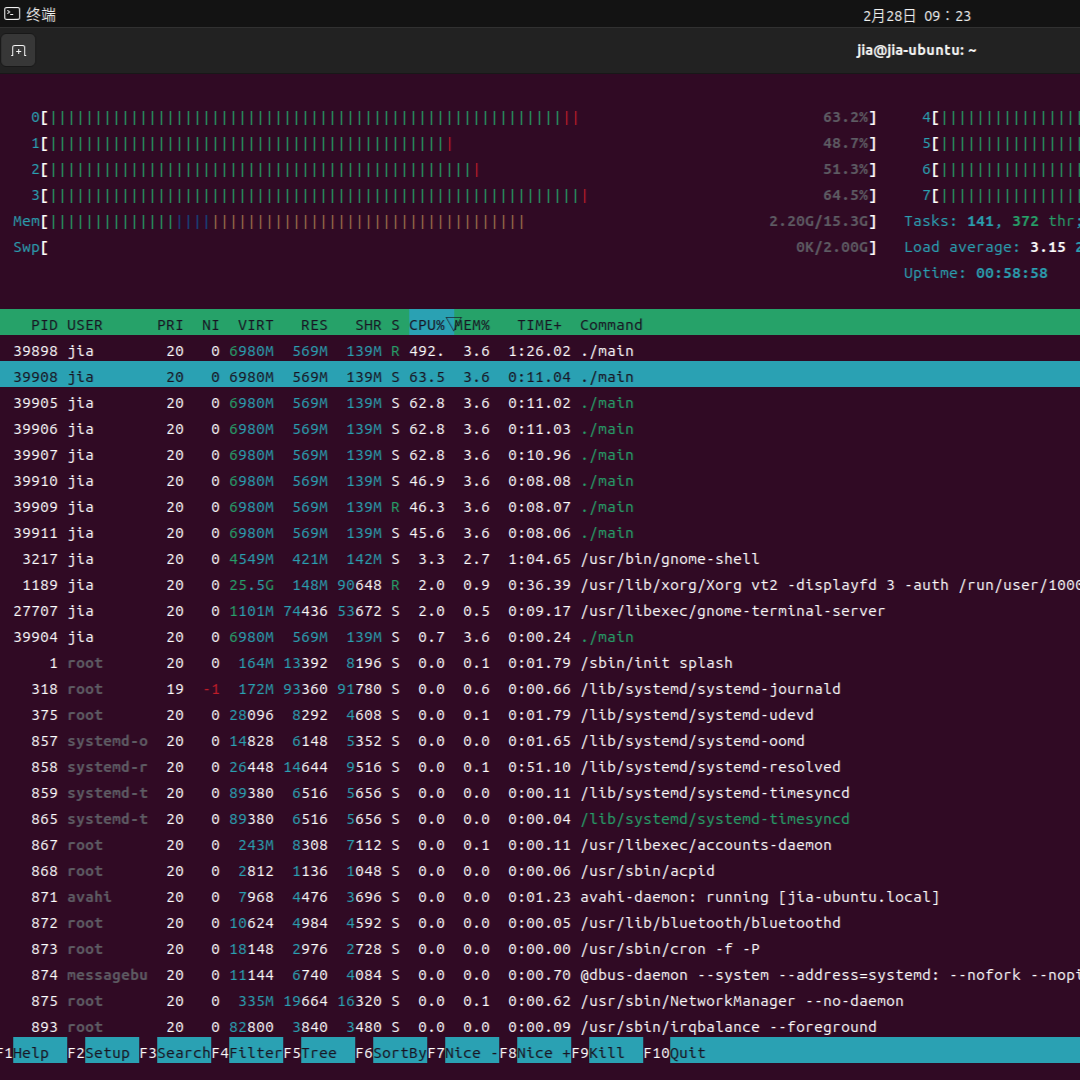
\includegraphics[width=1\textwidth]{figures/test_para/5cm_cpu.png}
		\end{minipage}
	}
	\subfigure[GPU]{
		\begin{minipage}[t]{0.48\linewidth}
			\centering
			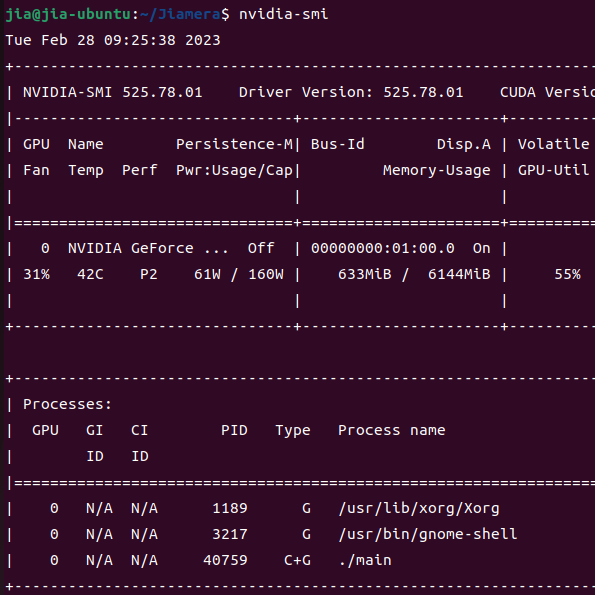
\includegraphics[width=1\textwidth]{figures/test_para/5cm_gpu.png}
		\end{minipage}
	}
	\caption{5cm点云分辨率性能占用}
	\label{fig:5cm_result}
\end{figure}

\paragraph{操作系统兼容性}
\par 系统在Windows平台运行良好,未出现兼容性问题;在Ubuntu平台除“\ref{vis_test}可视化模块”测试中所述问题外,无其他兼容性问题。

\paragraph{适应性}
\par 在处理不同规模的场景时,系统显示出良好的适应性。即使在处理大规模场景时,系统的性能也能保持在可接受的范围内。

\paragraph{安全性}
\par 由于采用单例模式,在长时间运行的测试中,没有发现内存泄漏问题。当设备断开连接或数据丢失时,系统进入循环等待状态,不会发生崩溃。

\paragraph{负载测试}
\par 在2 cm分辨率的环境下运行系统,系统仍然能够保持稳定运行。降至1.8 cm后,若不改变重建空间大小,内存会发生段错误。
点云分辨率与最大重建空间的对应关系见表\ref{table:size_space_relation}。

\begin{table}[htbp]
	\centering
	\caption{点云分辨率与最大重建空间对应关系}
	\label{table:size_space_relation}
	\begin{tabular}{m{3.5cm}m{1cm}m{1cm}m{1cm}m{1cm}}
		\toprule
		点云分辨率(cm)     & 1     & 2     & 4     & 8      \\
		\midrule
		最大重建空间($m^3$) & $2^3$ & $4^3$ & $8^3$ & $16^3$ \\
		\bottomrule
	\end{tabular}
\end{table}